\chapter{浏览器——网上冲浪必备}
\label{browsers-and-how-to-choose}

\begin{intro}
  浏览器是我们浏览网页的必备工具,它们将互联网上的形形色色的网页呈现在我们面前。
  不过,各种浏览器之间的门派以及它们之间交错复杂的历史渊源,却并不为多数人所知。
  
  通过阅读完这一部分,你也许可以找到下面这些问题的答案。
  
  \begin{itemize}
    \item IE 浏览器是何方神圣?
    \item Chrome 浏览器又是何方神圣?
    \item 火狐浏览器又是何方神圣?
    \item 「360 安全浏览器」「QQ 浏览器」「2345 王牌浏览器」都是怎么来的?
    \item 我应该选择什么浏览器?
  \end{itemize}
\end{intro}

浏览器是我们「网上冲浪」必备工具。
当你访问一个网站,比如说 \url{https://missing.criwits.top/},这个网站的内容就顺着网线和 Wi-Fi 传输到了你的设备(手机或电脑或其他)上。
浏览器所做的事情,就是将这些内容按它们所设计的样子「排版」或者说「呈现」,使其能完整、正确地展现在你的屏幕上。
同时,浏览器还负责与你进行交互:假如你点了一下这个网站上的某个按钮,浏览器就要去「理解」你的点击动作,并执行相应的功能。

\begin{figure}[htb!]
  \centering
  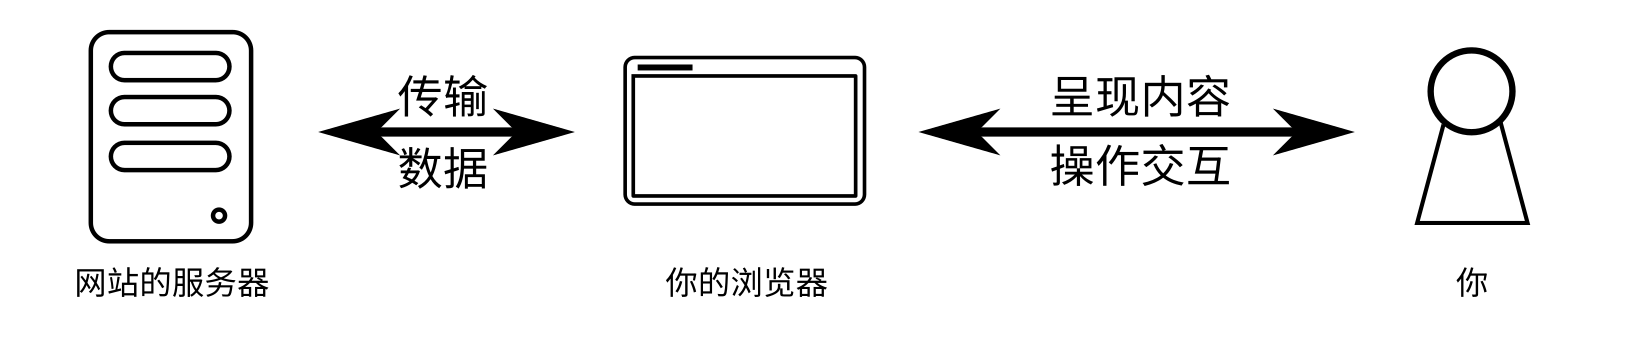
\includegraphics[width=12cm]{assets/How_Browsers_work.png}
  \caption{浏览器干的事}
  \label{How_Browsers_work}
\end{figure}

正如做数学题有人做得快有人做得慢,「排版」同一个网页,有的浏览器排得又快又好,有的则要花费更长的时间。
浏览器之间的最直观区别,就体现在同一网络下打开网页的不同速度上。
当然,不同的浏览器也有自己的特色,有的可以帮忙屏蔽一些广告,有的可以帮你记忆各种密码,有的能与「某某电脑管家」联动来保障安全,有的则只被用来下载其他浏览器。
「IE 浏览器」「火狐浏览器」「谷歌浏览器」「360 极速浏览器」「QQ 浏览器」……
这些名字或许你早已有所耳闻,但它们究竟孰优孰劣,可能还需要深入了解才能知晓。

\section{浏览器界的「血雨腥风」}

在讨论浏览器之前,我们可以先侃一侃「浏览器战争史」。

\subsection[第一次浏览器大战——网景和微软两大巨人的单打独斗]{第一次浏览器大战{\normalsize ——网景和微软两大巨人的单打独斗}}

让我们将时间的指针拨到 30 年前。
二十世纪九十年代,互联网刚刚进入民用领域,市面上开始出现各种各样的早期网络浏览器,它们的出现拉开了一场没有硝烟的「战争」的序幕。

\begin{wrapfigure}{r}{5cm}
  \centering
  
\includegraphics[width=4cm]{assets/Netscape.png}
  \caption{网景公司的 logo}
  \label{Netscape}
\end{wrapfigure}

这些早期网络浏览器的作者中,有一个叫马克·安德森的人比较有商业头脑——他嗅到了互联网时代的机遇。
1994 年,他和自己的伙伴成立了「网景通讯」公司,并推出了一款商业化的浏览器软件——「网景浏览器」。
网景浏览器以「共享软件」的方式运作——即软件本身需要交钱购买,但是可以先免费试用。
由于网景浏览器相比竞品(虽说那时本来也没什么竞品)更加实用、稳定,网景很快统领了浏览器的市场,并成为了互联网领域的「绝对标准」。

微软见网景在互联网领域如鱼得水赚了大钱,心里很不是滋味,于是也想在浏览器领域分一杯羹。
1995 年,微软发布了「Internet Explorer」,它简写来就是「IE」。
IE 在一开始并没有取得什么竞争上的优势——一开始,它不如网景浏览器稳定,有着更多的安全漏洞并更容易死机。
但到了 1997 年,微软发布 IE 4.0,这个版本的 IE 做了几件大事:
一是\regcolor{它变成了 Windows 系统中的一部分}\CJKsout*{(捆绑安装)},二是它终于做得比网景更好了。
自此之后,IE 迅雷不及掩耳地抢占了大量市场份额。
到了 1998 年,网景被 AOL 公司收购,原来的浏览器开发团队也解散了。

至此,微软在这一场与网景的较量之中胜出,IE 浏览器成为了浏览器界的老大,第一次浏览器大战结束。

\begin{figure}[htb!]
  \centering
  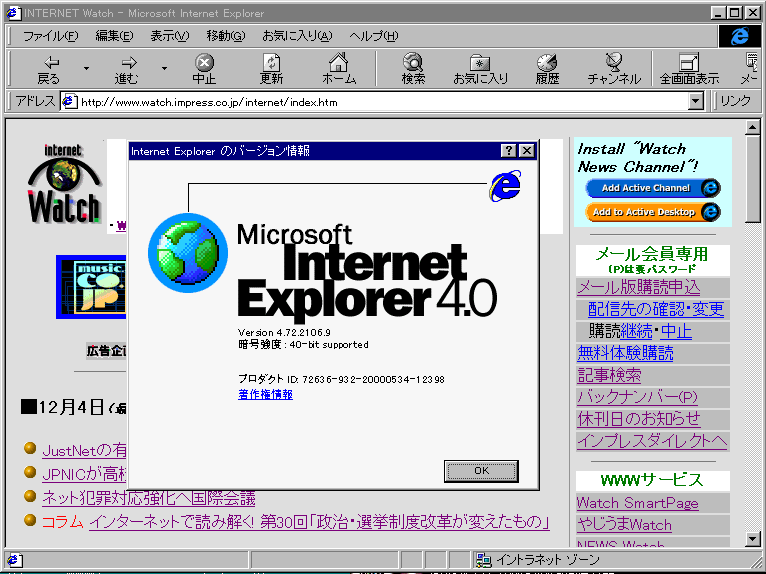
\includegraphics[width=10cm]{assets/IE_4.png}
  \caption{IE 4.0 的界面}
  \label{IE_4}
\end{figure}

\subsection[第二次浏览器大战——开放、自由的竞争与新时代的机遇]{第二次浏览器大战{\normalsize ——开放、自由的竞争与新时代的机遇}}

网景虽然在第一次浏览器大战中惨败,但它并没有立刻退出这个市场,而是希望联合更多的力量来抗衡自己的对手。
1998 年,也就是网景被收购的那年,它公开了自己的网景浏览器的源代码,成立了以 Mozilla 为名的开发社团,希望借助更多人的力量将这一股薪火传下去。

时间来到 2003 年,苟延残喘的网景公司最终解散。
解散当天,AOL 也分离了与 Mozilla 的关系,Mozilla 成为了一个独立的「基金会」。
所谓「基金会」,就是说自身不以营利为目的,而依赖社区——或者说大众——的力量进行开发,依赖用户的捐赠来维持运行。
不久后,Mozilla 将自己开发的,「传承」自网景的浏览器赋予「Firefox」的名字,即「火狐」。
由开放社区贡献的火狐得到了人们的认可,数年间就占领了超过 20\% 的浏览器市场。
下图是自 2004 年以来火狐浏览器的图标变化。

\begin{figure}[htb!]
  \centering
  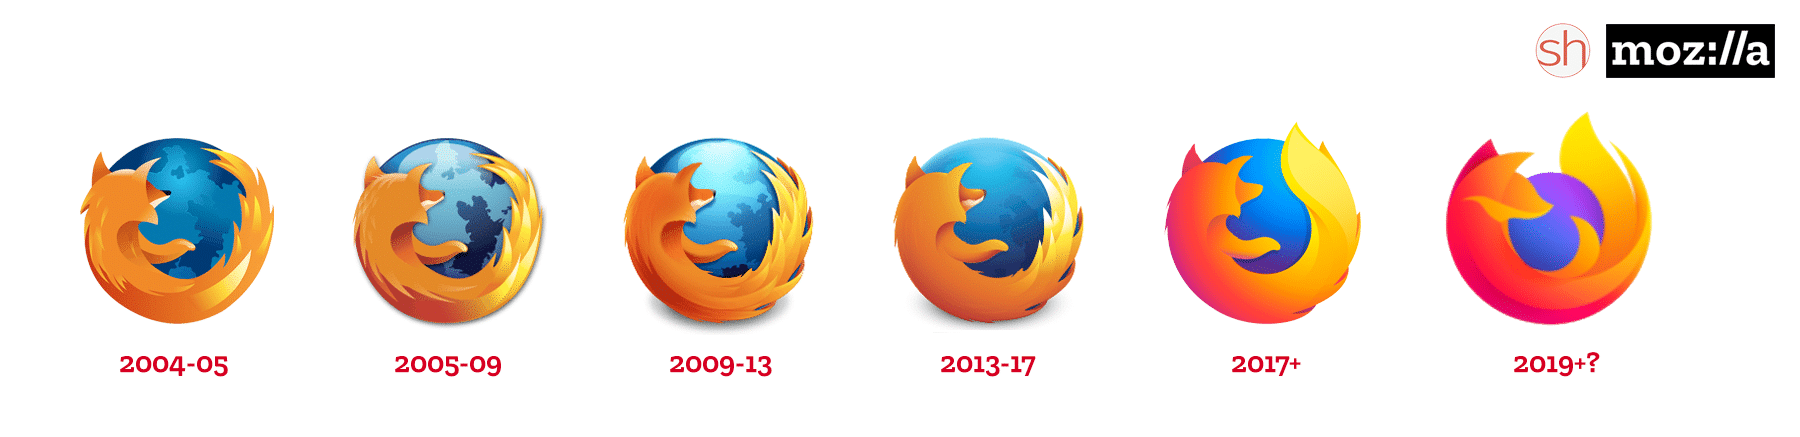
\includegraphics[width=12cm]{assets/Firefox_Logo_History.png}
  \caption{火狐浏览器的图标变化}
  \label{Firefox_Logo_History}
\end{figure}

微软见火狐迅速占领市场,来者不善,于是着手为 IE 添加新的功能,以让它能与火狐抗衡。
2006 年,微软发布了 IE 7,在界面和功能上都有了许多改变,但却在性能上惨不忍睹,在新标准支持方面也实在难以恭维。
又由于为 IE 7 护航的 Windows Vista 实在太拉,IE 7 几乎没有取得什么成功。
后来的 IE 8 尽管做了很大改进,但在新标准支持方面仍然表现差劲,与竞争对手间存在很大的差距。
IE 的市场份额因而不断走向下坡,而火狐的占有率则在 2008 年前后冲上了 30\% 的高峰。

\begin{figure}[htb!]
  \centering
  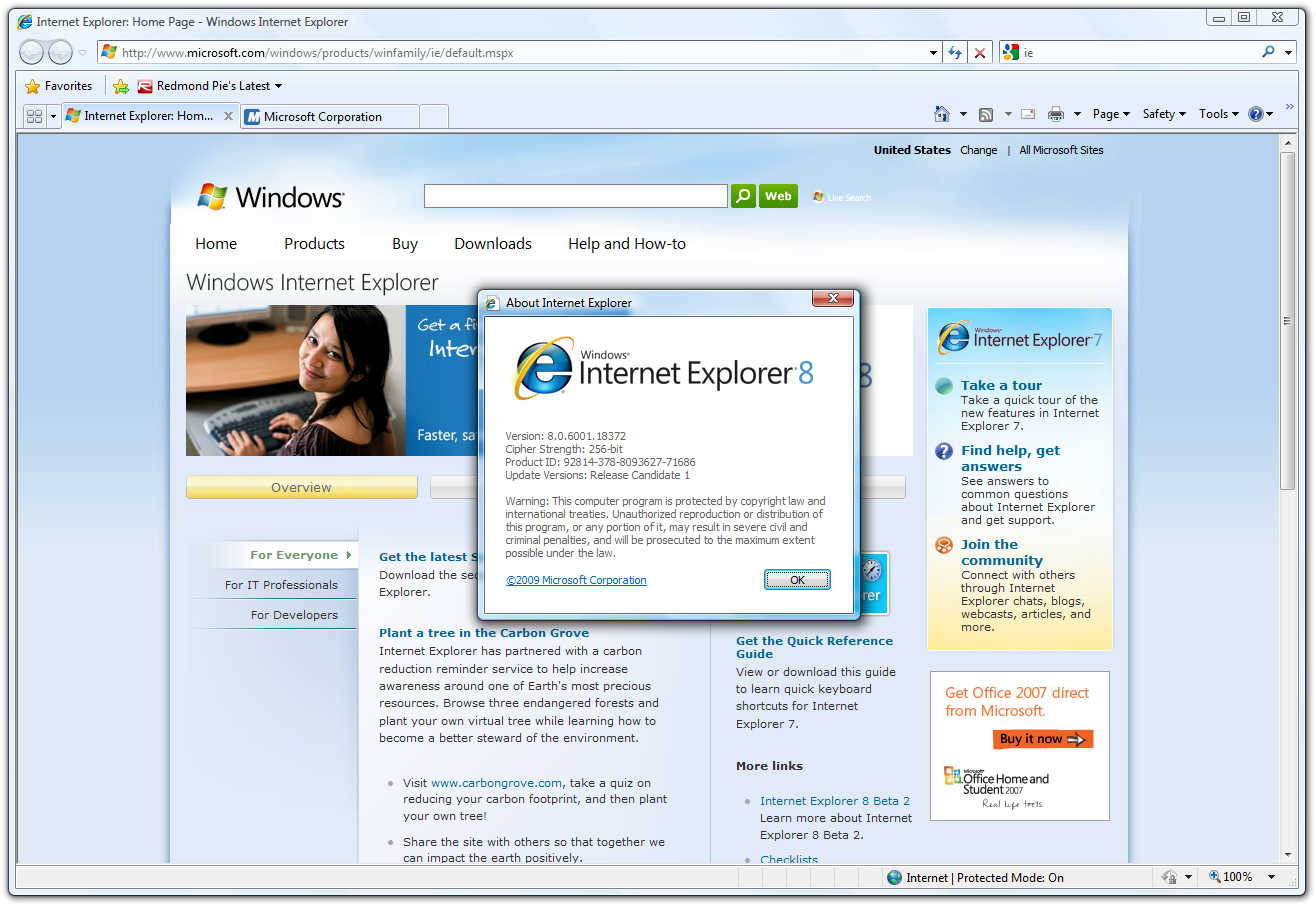
\includegraphics[width=10cm]{assets/IE_8.png}
  \caption{IE 8 的界面}
  \label{IE_8}
\end{figure}

与此同时,越来越多的企业和组织意识到了浏览器市场的重要性。
除了 Mozilla 的火狐和微软的 IE 外,其他许多竞争者也参与到了这场新的浏览器大战中。
2008 年,谷歌公司\CJKsout*{(也就是某个官网都打不开的公司)}推出了一款全新浏览器——Chrome 浏览器,也就是我们俗称的「谷歌浏览器」。
下面展示的是今天 Chrome 浏览器的画面。

\begin{figure}[htb!]
  \centering
  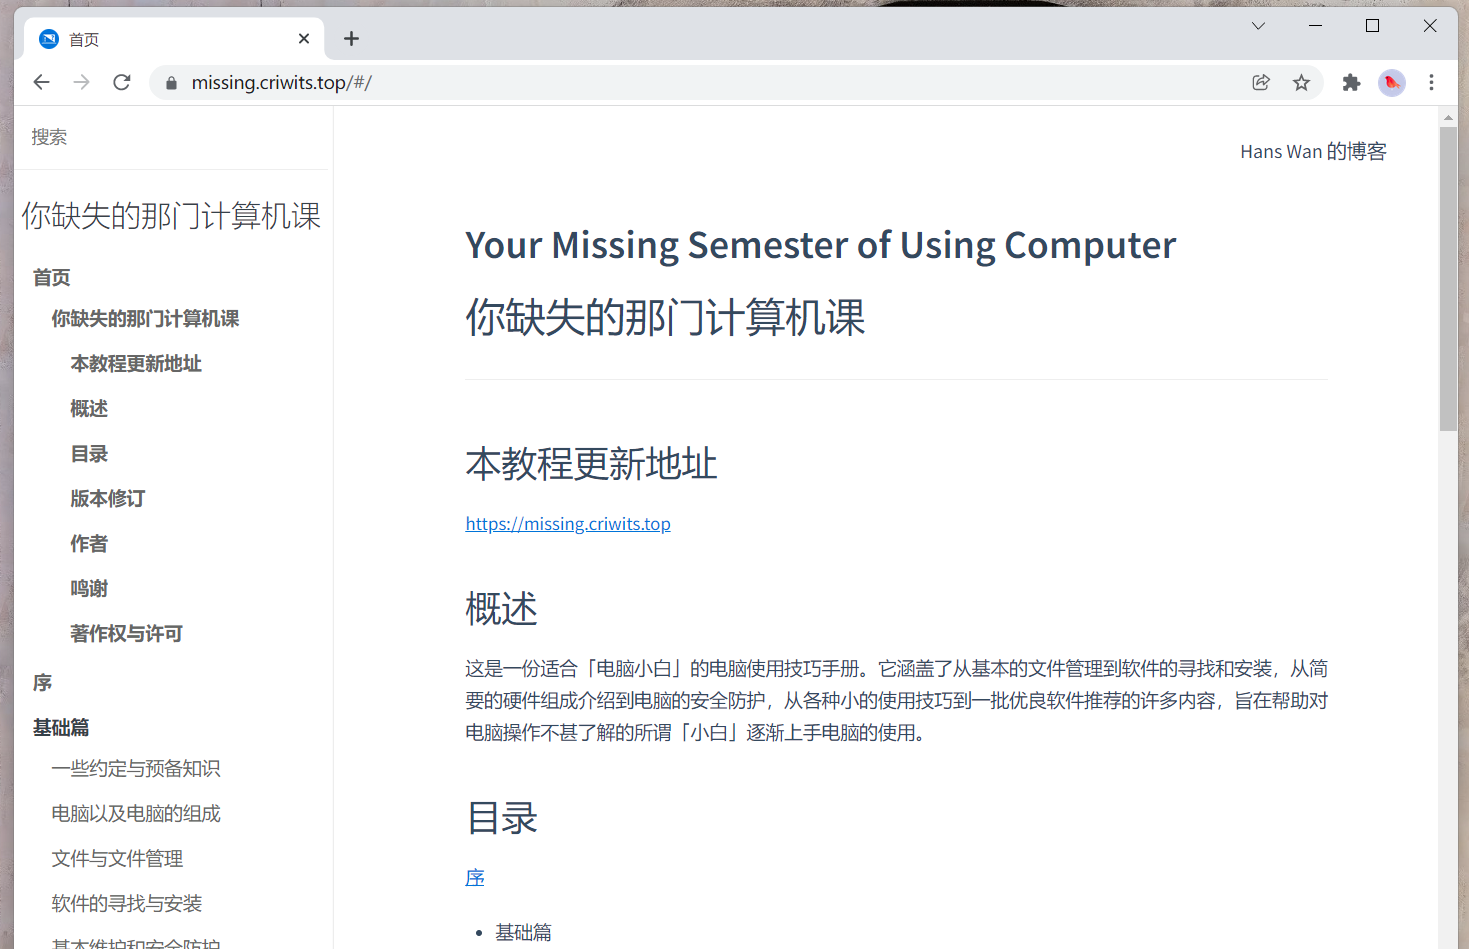
\includegraphics[width=9cm]{assets/Chrome_Example.png}
  \caption{如今 Chrome 的界面}
  \label{Chrome_Example}
\end{figure}

Chrome 浏览器诞生不久就开始迅猛发展并占领市场。
这有着多方面的原因:
第一,谷歌公司自身的体量强大,因而能够借助自己的网络生态——例如谷歌搜索、谷歌邮箱(Gmail)等访问量巨大的网站——来「助推」Chrome 浏览器。
第二,谷歌的确投入了人力物力进行 Chrome 浏览器的开发,一直以来,Chrome 浏览器在性能上与竞争对手相比都有着不小的优势。

\begin{note}
  另一个重要原因是,Chrome 浏览器诞生的年代(2010 年前)正好是赶上了互联网从原来的单一化向多元化发展的时代大潮。
  而 Chrome 对那时产生的一系列新标准和规范有较好的支持,可以说是一直赶在时代潮头;
  相比之下,由于微软的 IE 浏览器是与 Windows 系统捆绑更新的,而 Windows 系统数年才发布一个新版本,再加上 IE 无论是性能还是功能都不断地落后于其他浏览器,IE 的市场占有率自那时开始就持续走低。
\end{note}

前面我们提到过,火狐浏览器是「开源」的软件,它的源代码自诞生以来一直都是公开的——这意味着,任何人都可以在遵守一定约定的前提下,自由地修改和发布它。
这样,火狐浏览器就能「集思广益」,以社区之力推进开发。
谷歌看到了这种模式的优势,但又不想让自己的得意之作完全被众人窥探,于是谷歌想了个办法,它将 Chrome 浏览器的核心部分拿出来,以「Chromium」这个名字开源。
顺带说一句,「Chrome」是「铬金属」,「Chromium」是「铬元素」,外在与内核,正是照应了它们的名字。
有了 Chromium,社区大众可以拿它去进行二次开发和改进,谷歌则将这之中的开发进展不断地吸收回 Chrome。
这样就形成了一个由开放的 Chromium「反哺」封闭的 Chrome 的过程。
如果你正在使用 Chrome 浏览器,不妨打开【设置】→【关于 Chrome】,你就能看到这样一句话:「Chrome 的诞生离不开 Chromium 开源项目以及其他开源软件」。

\begin{figure}[htb!]
  \centering
  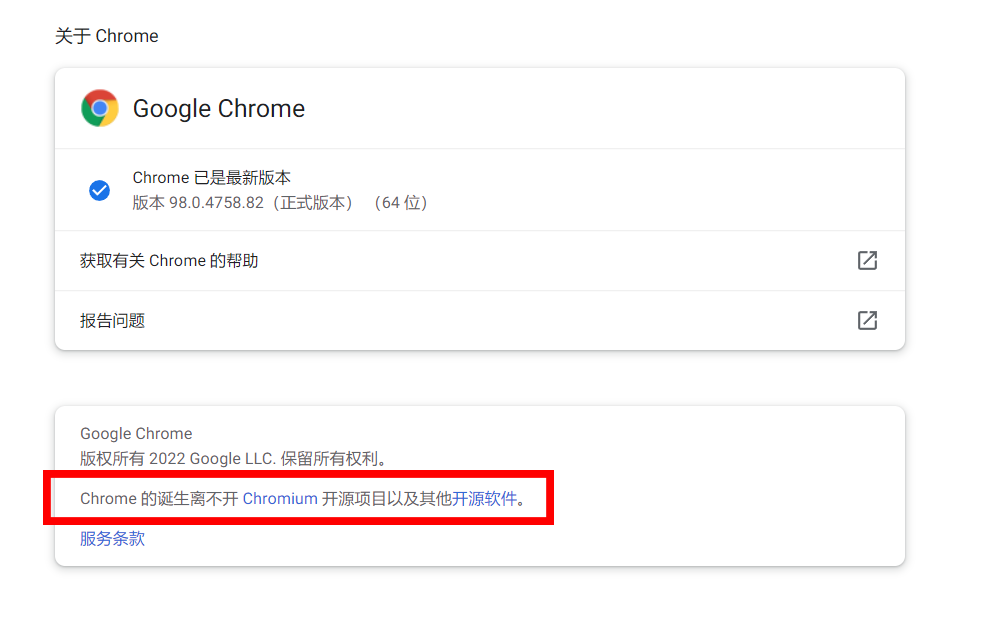
\includegraphics[width=9cm]{assets/About_chrome.png}
  \caption{【关于 Chrome】}
  \label{About_chrome}
\end{figure}

众所周知,Chrome 浏览器好用,而谷歌又把它核心部分给公开了,这让许多其他厂商有了新的想法:
从零开始重新设计一个浏览器实在太难,但浏览器着实赚钱(主要是广告效应,以及可以借浏览器来推广自家的其他功能),不如就把这 Chromium 借来,套上一个外壳,做成自己的浏览器好了。
由于国内特殊的网络环境,谷歌的一些服务在大陆无法使用,这更给予了国内一些互联网大厂打造自己浏览器的动力。
「360 极速浏览器」「QQ 浏览器」「2345 王牌浏览器」「世界之窗浏览器」等这些国产浏览器,都是在 Chromium 的基础上「套壳」而来的产物
——它们都使用者和 Chrome 一样的核心技术,只是披上了不同的外衣,附加了各自的独有功能,比如「网络安全」「账户同步」等。
在这些浏览器的有关页面上,我们也都能找到它们与 Chromium 的关系。例如,下图是 360 极速浏览器的介绍页,这里的「Chrome 内核」指的就是 Chromium。

\begin{figure}[htb!]
  \centering
  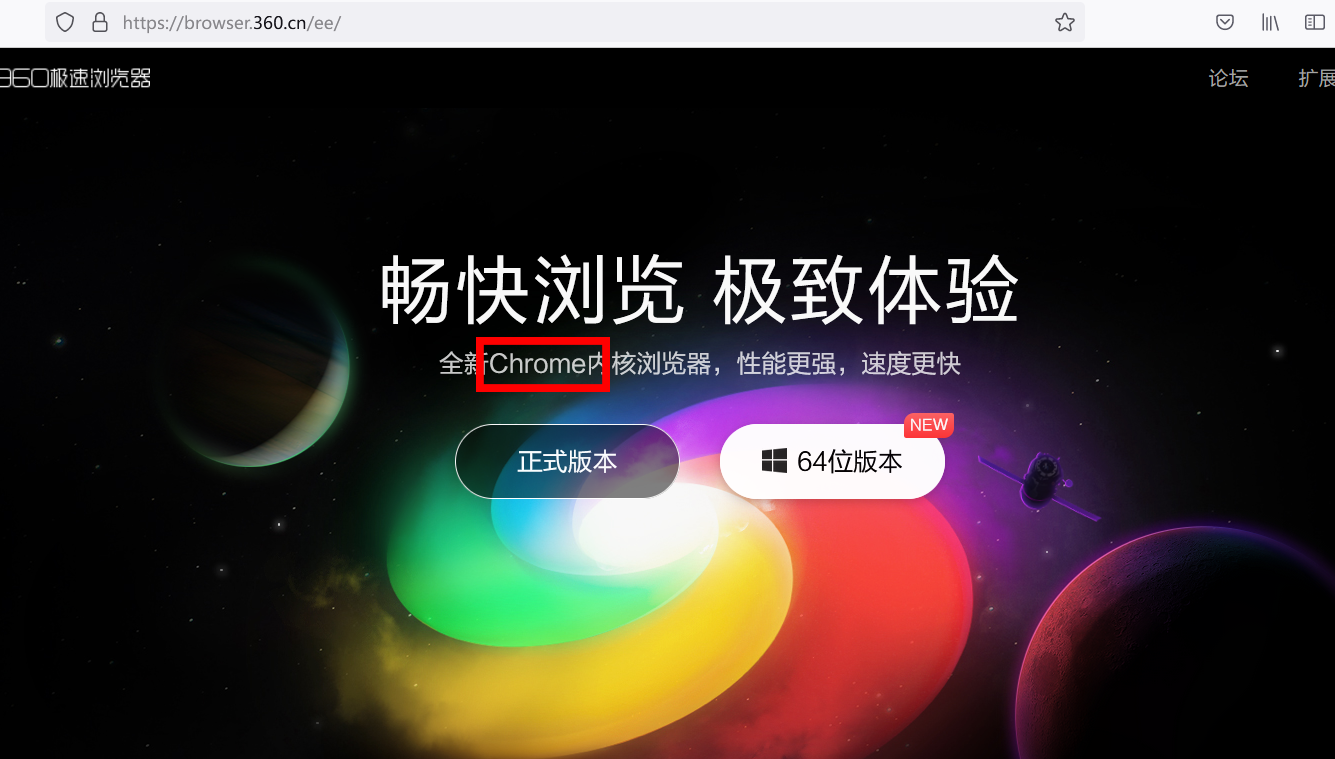
\includegraphics[width=8cm]{assets/360_ee.png}
  \caption{360 极速浏览器}
  \label{360_ee}
\end{figure}

再比如说,QQ 浏览器的官网上,硕大的「CHROMIUM」标榜着自己的内核\CJKsout*{(不过现在 Chromium 都版本 97+ 了你怎么还在用 70 啊?)}:

\begin{figure}[htb!]
  \centering
  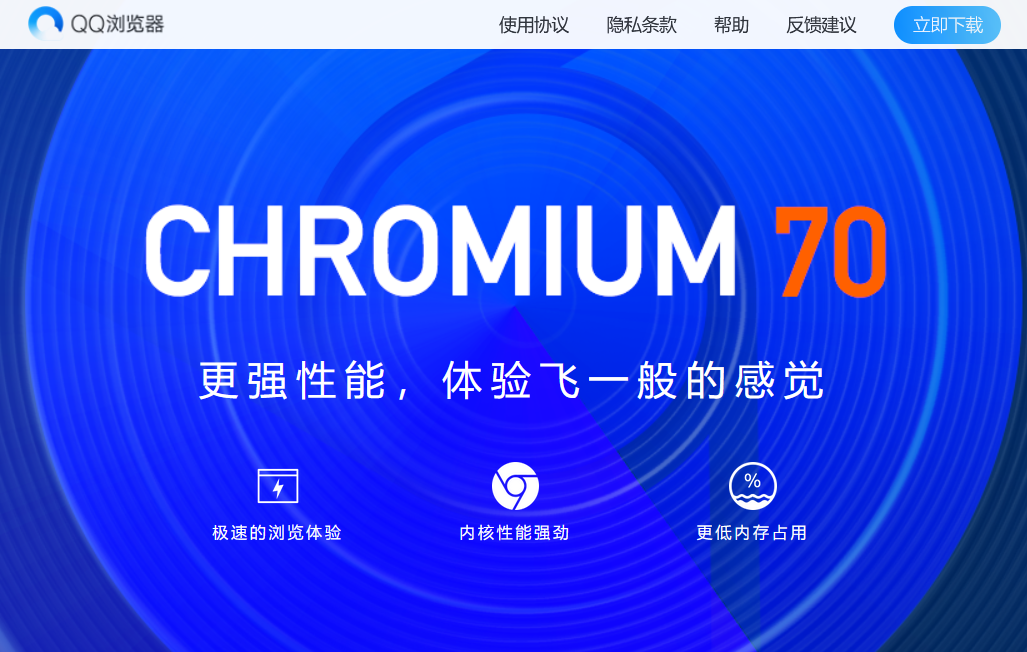
\includegraphics[width=8cm]{assets/QQ_Browser.png}
  \caption{QQ 浏览器}
  \label{QQ_Browser}
\end{figure}

就连微软——又是你微软——也在最后走上了套壳 Chromium 的道路。
先回头看看 IE 浏览器,它自 2013 年的 IE 11 以来就没有再更新过大版本。
倒是在 2015 年前后,微软发布了一款新的浏览器「Edge」,彼时的 Edge 还是在 IE 的基础上开发的,可以算是 IE 的正统后继者——连 IE 的缺点也一并后继了。
于是之后几年,Edge 一直不温不火,尽管它和 Windows 10 捆绑,但市场占有率一直比较低迷。
\CJKsout*{毕竟 IE 是什么乐色大家都懂,那几年的 Edge 只能说稍微比过去的 IE 好那么一丁点。}

\begin{wrapfigure}{r}{6cm}
  \centering
  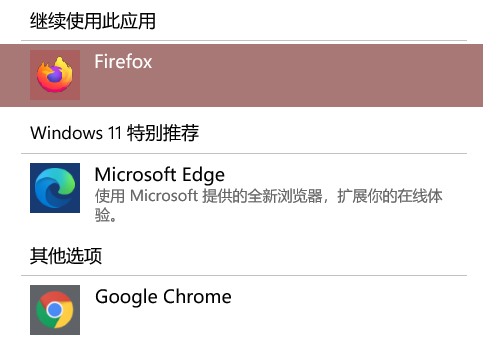
\includegraphics[width=5cm]{assets/Recommend_Edge.png}
  \caption{「来试试Edge吧!」}
  \label{Recommend_Edge}
\end{wrapfigure}

时间一转眼到了 2018 年。
那年末,微软搞了一个大新闻,要将 Edge 迁移到 Chromium 内核——换句话就是,把 Edge 原来的技术扔掉不要,新的 Edge 将是一款 Chromium 套壳的浏览器。
新 Edge 最终在 2020 年正式问世,全称「Microsoft Edge」。
这或许是微软的一次翻身——近两年,Edge 浏览器的市场份额开始稳步上升,一方面得益于 Chromium 内核的强大,另一方面则是微软借 Windows 来强行推荐 Edge。
如果你使用的是 Windows 10 或 11,你一定在系统的许多地方都能看见微软强行推荐 Edge 的身影,就如图 \ref{Recommend_Edge} 一样。

而 IE 真的成为弃子了。
2021 年 5 月 20 日,微软官宣即将停止支持 IE 浏览器,IE 将于 2022 年 6 月 15 日彻底「退役」。
诞生于第一次浏览器大战的 IE 在那时碾压对手网景,却最终在第二次浏览器大战中成为历史。
在今天,除了因国内有一些网站,例如「工行网银」「个人征信中心」等由于这样那样的历史原因必须要使用 IE 浏览器才能正常工作外,我们已经没有任何理由去使用 IE 浏览器。

Chrome 很优秀,这让 Chromium 套壳的浏览器,例如「360 极速浏览器」都有相对不错的用户体验,再加上这些做套壳的厂商一般都会在浏览器中附加一些自己设计的小功能,让它们在一定程度上更易于使用,Chrome 系浏览器(包括新 Edge)的市场份额在近年来已经差不多 70\%。
说 Chrome 垄断了浏览器市场,一点也不为过。
下图是自 2009 年至今的全球电脑端浏览器份额曲线图,其中绿线是 Chrome 以及 Chromium 套壳浏览器。

\begin{figure}[htb!]
  \centering
  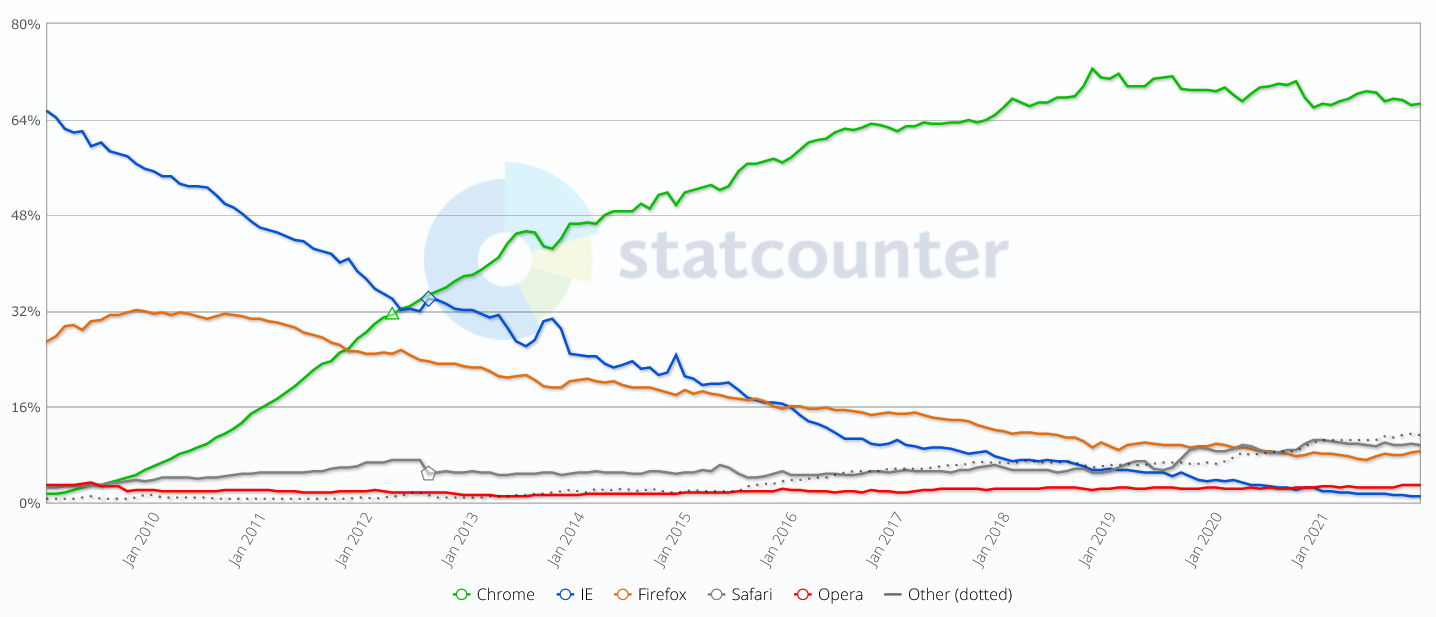
\includegraphics[width=11cm]{assets/Desktop_Browser_Market.png}
  \caption{电脑端浏览器市场份额}
  \label{Desktop_Browser_Market}
\end{figure}

与此同时,火狐——火狐是独立的、不同于 Chromium 的内核——的日子变得不太好过了。
在 2010 年之前,火狐的市场份额还比较高,且有上升迹象,但在 Chrome 大行其道后就开始逐步下降。
虽说火狐在性能上不差,但很多时候还是比不过 Chrome,再加上火狐毕竟是「用爱发电」,在宣传等方面肯定不如谷歌以及那些套壳大厂来得猛。
如今,火狐只剩下不到 10\% 的市场占有率。

\regcolor{第二次浏览器大战的余波至今仍未平息,并且是以 Chrome 的碾压性胜利在继续。}
在这 20 年间,我们见证了 IE 的衰亡、Edge 的新生、火狐的起伏、Chrome 的高歌;
以及谷歌的迅速入市、发展和壮大,微软的不断尝试、碰壁和迂回。
在互联网时代,市场需求瞬息万变,科技进步日新月异,浏览器之间的竞争背后,实则是技术和资本的较量。
未来何去何从我们不得而知,但希望你读到这里时没有昏昏欲睡。

\section{Chrome:一直被模仿,从未被超越}

Chromium 套壳千千万,但我们始终最推荐 Chrome 自身,正所谓「一直被模仿从未被超越」。

\begin{figure}[htb!]
  \centering
  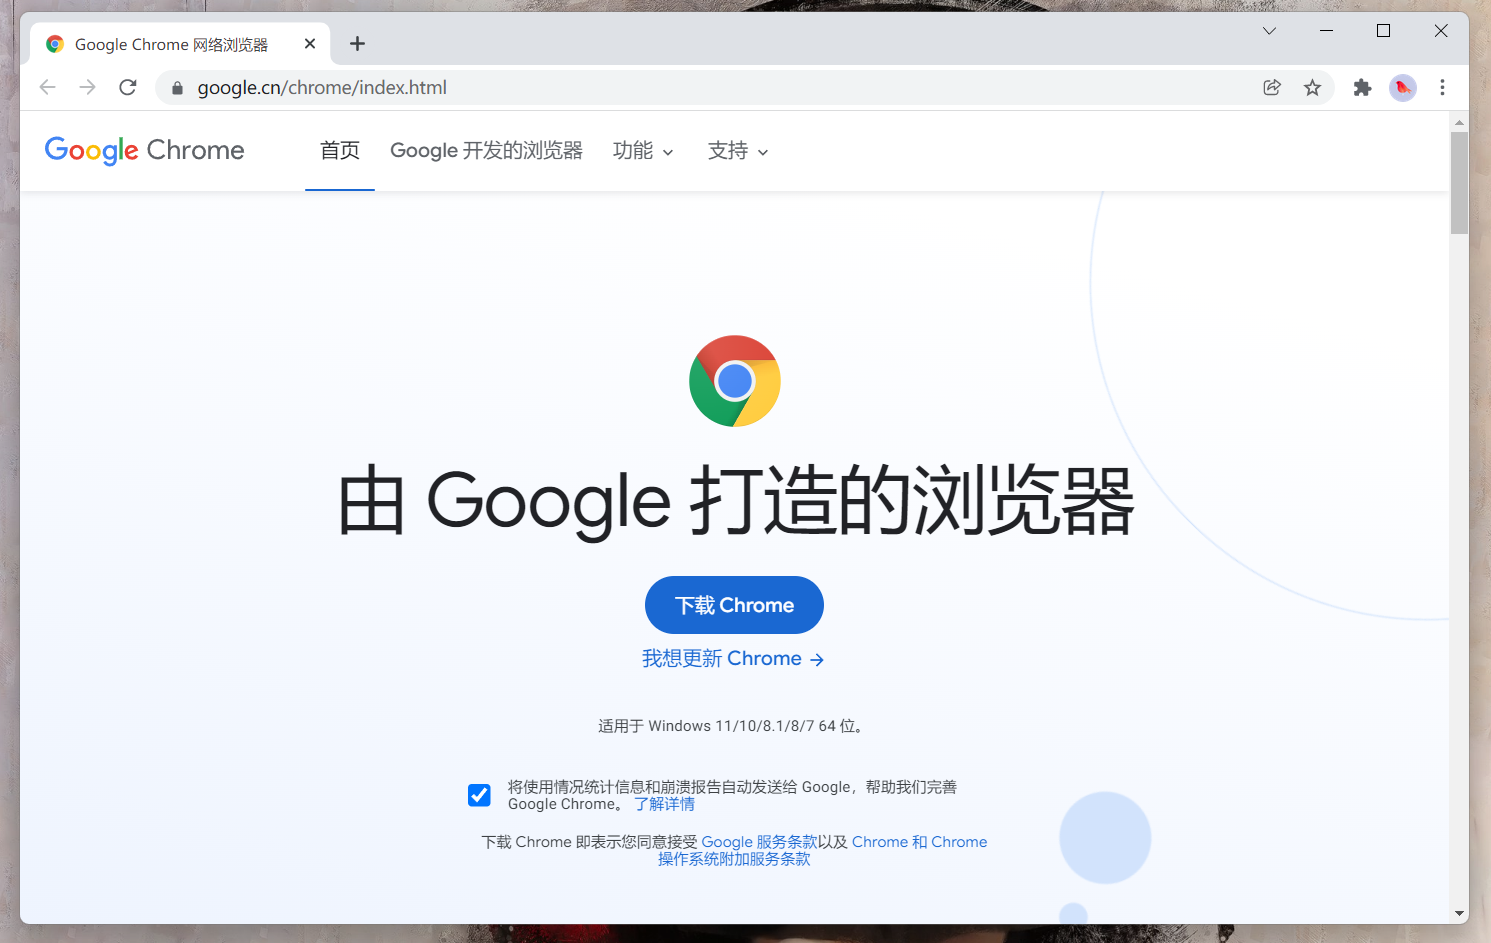
\includegraphics[width=10cm]{assets/Chrome.png}
  \caption{Chrome}
  \label{Chrome}
\end{figure}

Chrome 性能出色,界面干净简洁,没有多余繁杂的功能栏,设计优雅美观。
Chrome 稍微影响使用的缺点,可能是在国内无法稳定地使用「同步」等功能。
这「同步」功能,是指在浏览器上登录自己的账号之后,就能同步自己的收藏夹、历史记录、密码本等数据,实现多设备联动。
由于 Chrome 的老东家是谷歌,而谷歌服务无法正常在大陆地区访问,这造成一般情况下我们只能不登录使用 Chrome。
不过,在自己对同步功能依赖不深的情况下,这一缺点也是可以忽略的。

Chrome 浏览器的官方下载地址是 \url{https://www.google.cn/intl/zh-CN/chrome/}。
此链接是可以在中国大陆地区直接访问并正常下载的。
下载安装之后的 Chrome 也是可以正常在中国大陆地区更新的。
\CJKsout*{(难能可贵难能可贵)}

\section{Firefox:星星之火,正将燎原}

Firefox——或者说火狐——是今天 Chrome 垄断浏览器市场背景之下还在「坚守」的浏览器之一。

\begin{figure}[htb!]
  \centering
  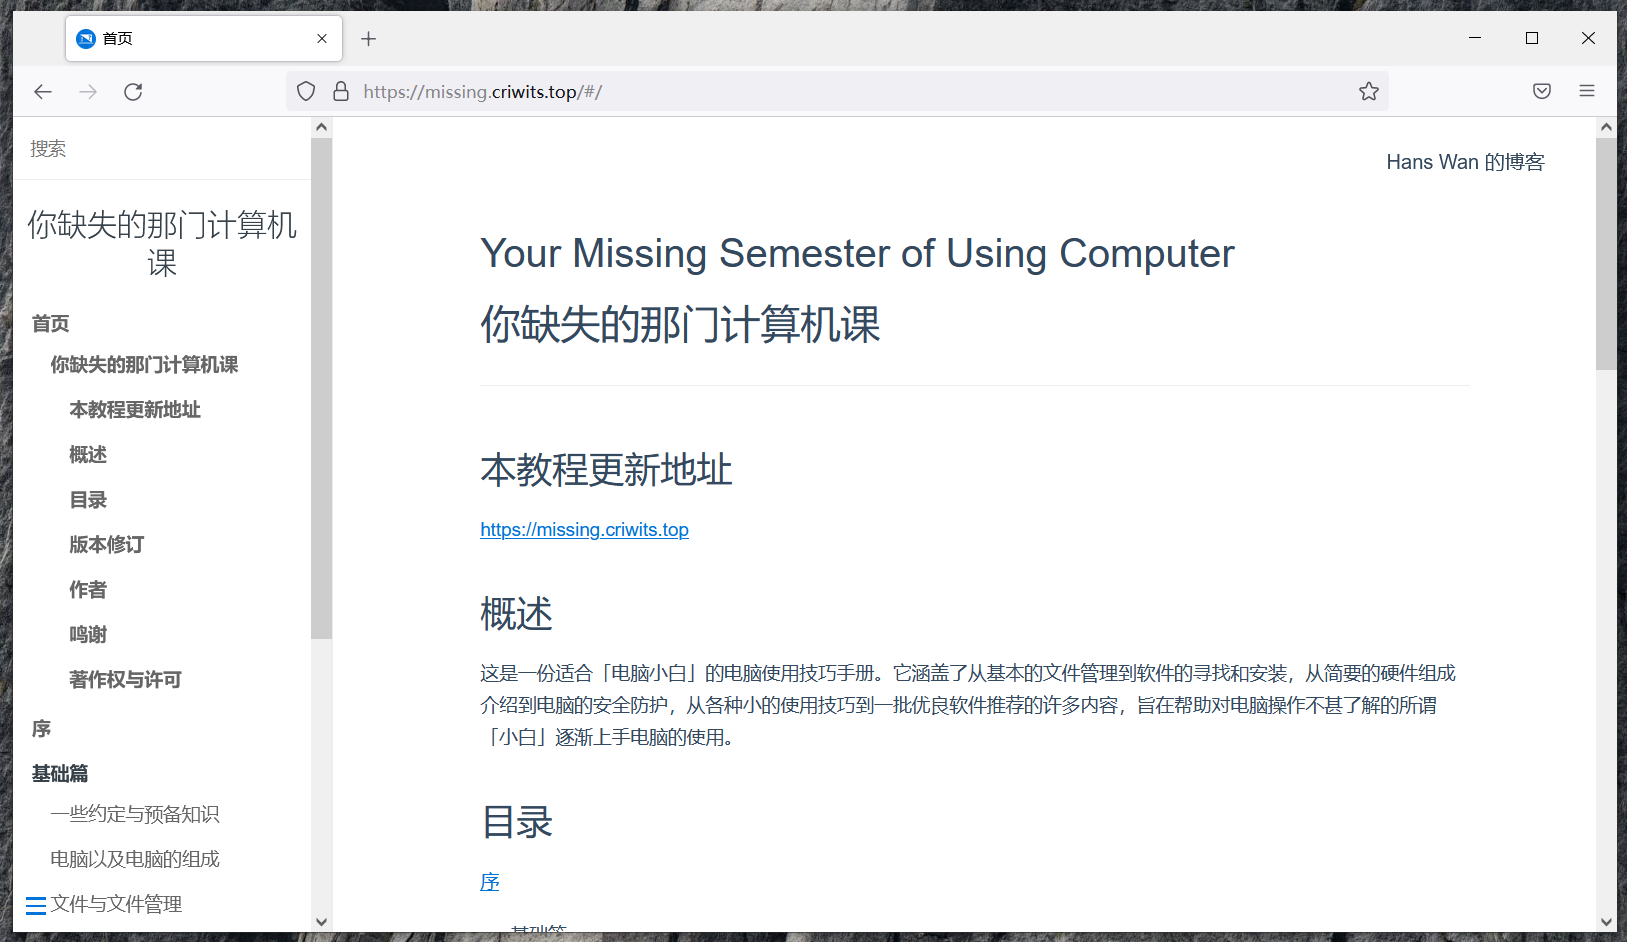
\includegraphics[width=10cm]{assets/Firefox.png}
  \caption{Firefox}
  \label{Firefox}
\end{figure}

Firefox 的性能稍弱于 Chrome,不过差距并不大。
在界面上,Firefox 同样设计得较为合理美观。
Firefox 是可以在国内正常使用同步功能的。
具体来说,在国内能够下载到的 Firefox 有两个版本:

\begin{itemize}
  \item 国际版 Firefox,即全球通用的 Firefox,从 Firefox 国际官网上下载到的 Firefox 就是这个版本。
    使用国际版 Firefox 的同步功能时,你的账号和数据可能会存储在国外。
    国际版 Firefox 可以正常在国内使用同步等功能。
  \item 中国版 Firefox,是由国内与 Mozilla 的合资公司发行的针对中国市场供应的 Firefox。
    与国际版 Firefox 最大的不同是,使用中国版 Firefox 的同步功能时,你的账号和数据会存储在国内。
    这是因为我国法律出于国家安全的考量,要求在国内落地的互联网服务提供商不能把用户的数据存储在境外,但用户可以自己选择使用国内或国外的产品。
\end{itemize}

国际版 Firefox 可以在 \url{https://www.mozilla.org/zh-CN/firefox/new/} 下载到;
中国版 Firefox 可以在 \url{https://www.firefox.com.cn/} 下载到。
我们偏向更推荐使用国际版 Firefox,尽管二者在功能和性能上并无二致(中国版 Firefox 内置了一些所谓的「实用插件」,但都没什么用)。

\section{Edge:微软最后的妥协}

这里的「Edge」说的是使用 Chromium 内核的新 Edge,它的图标蓝中带点绿。
老 Edge 的图标是蓝色的「e」,不过今天已经不容易见到,因此这里不考虑它。

\begin{figure}[htb!]
  \centering
  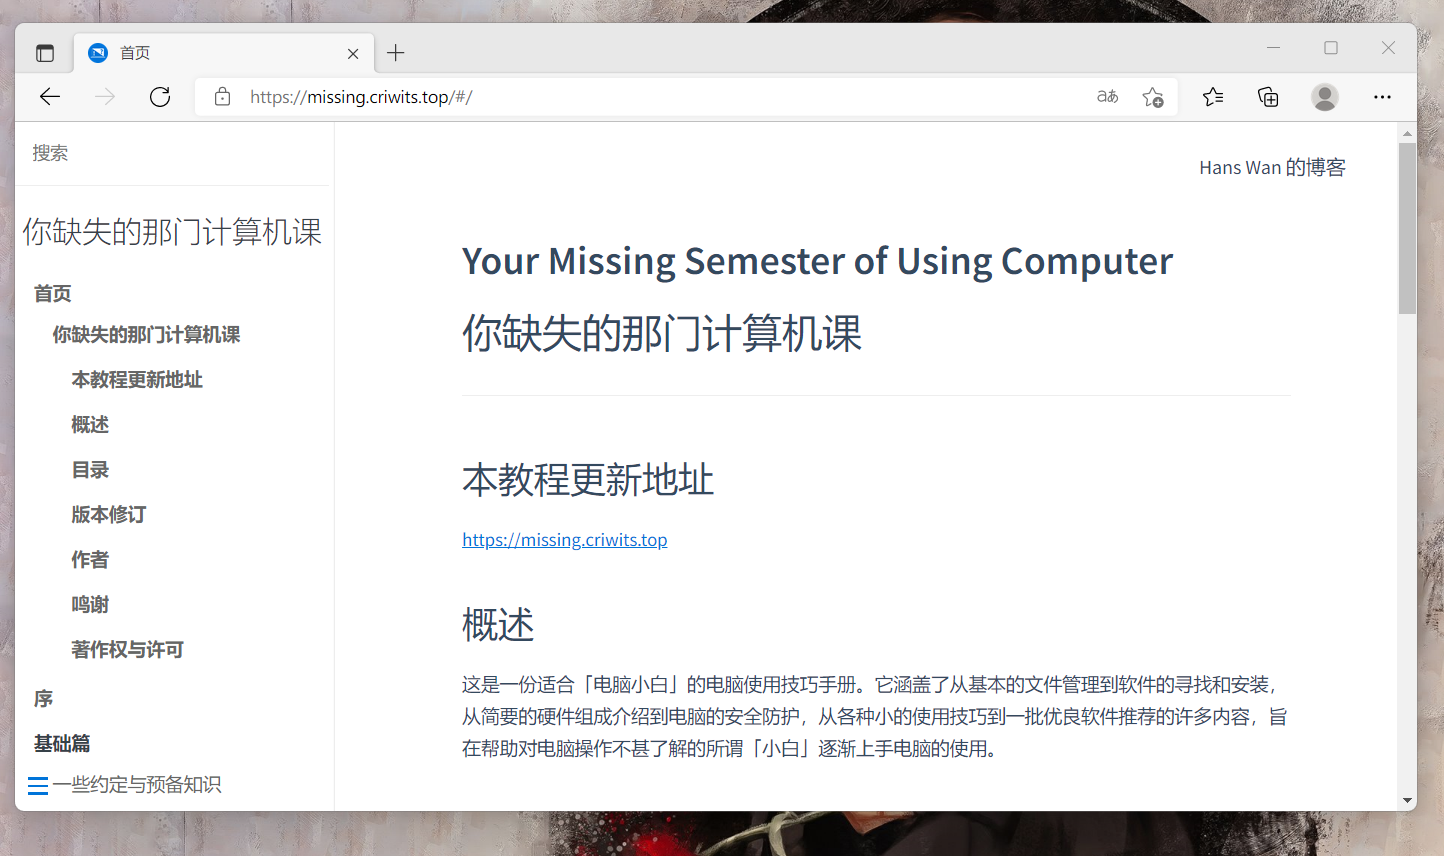
\includegraphics[width=10cm]{assets/Edge.png}
  \caption{Edge}
  \label{Edge}
\end{figure}

由于使用了 Chromium 内核,新 Edge 的性能自然和 Chrome 站到了同一梯队。
在外观上,新 Edge 和 Chrome 基本一致,但加入了一些比较有用的小功能,例如「垂直标签页」等。
Edge 使用微软账号登录,因而也能在国内正常同步。
对于想使用 Chrome 却苦于同步等功能的用户来说,新 Edge 是他们非常不错的一个选择。

新 Edge 在现在的 Windows 10 或 11 系统中预置,打开即可使用;
如果你想下载安装,可以访问 \url{https://www.microsoft.com/zh-cn/edge} 来下载。

\section{IE:也许你还用得到}

\begin{wrapfigure}{r}{6cm}
  \centering
  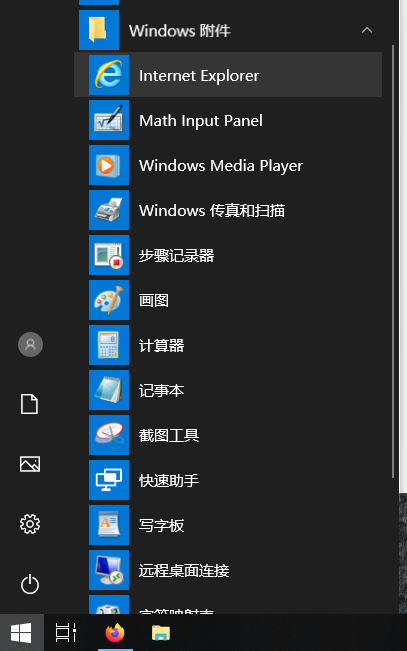
\includegraphics[width=5cm]{assets/IE_on_Win_10.png}
  \caption{Windows 10 中的 IE}
  \label{IE_on_Win_10}
\end{wrapfigure}

上文中说过,国内有些网站必须要用 IE 浏览器才能工作。
「这样那样的历史原因」便是:这些网站开发得比较早,在那时 IE 还大行其道,因此它们的一些特殊功能(主要是安全相关的功能)是针对 IE 浏览器的部分专有特性开发的。
如上文所言,后来斗转星移,IE 最终退出了这个时代,但那些网站却没来得及更新技术。
这些网站主要有工商银行网银平台、中国人民银行征信平台、教师资格证报名平台等。

在 Windows 10 系统中,IE 11——也就是 IE 的最后一个版本——得以作为系统的一部分而保留。
你可以通过【开始】→【Windows 附件】→【Internet Explorer】来打开它,如图 \ref{IE_on_Win_10}。

当然你也可以打开「开始菜单」后,直接键入「Internet Explorer」来找到它。

而在 Windows 11 中,IE 已经被移除出系统。
在这种情况下,如果网站要求使用 IE 浏览器,你可以尝试使用 Edge 的「IE 模式」。
具体来说,你需要首先打开 Edge 并进入「设置」(右上角【⋯】→【设置】),然后选择【默认浏览器】,将「允许在 Internet Explorer 模式下重新加载网站」设置为【允许】,如图 \ref{Edge_IE_Mode_1}。

\begin{figure}[htb!]
  \centering
  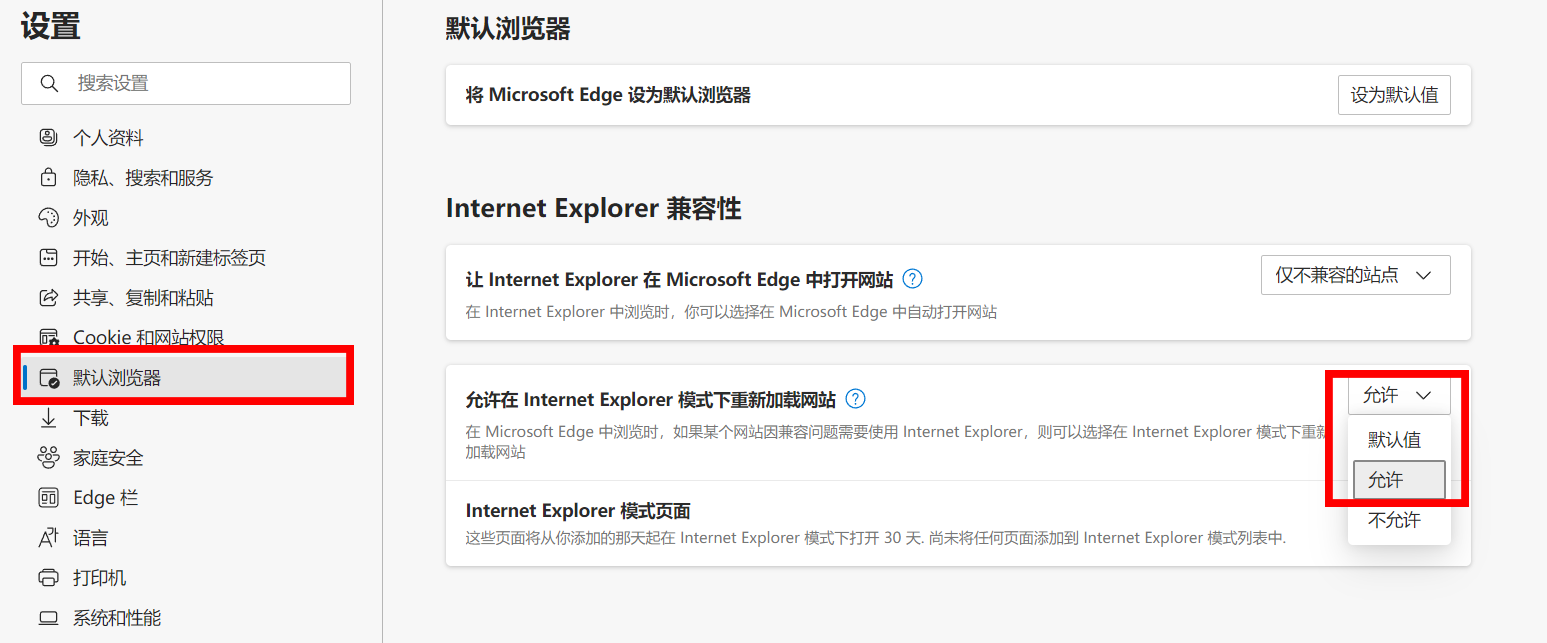
\includegraphics[width=10cm]{assets/Edge_IE_Mode_1.png}
  \caption{启用 Edge 的 IE 兼容}
  \label{Edge_IE_Mode_1}
\end{figure}

设置完之后关闭 Edge 再重新打开。
然后,用 Edge 打开你需要用 IE 打开的网页,点击右上角【⋯】并选择【在 Internet Explorer 模式下重新加载】,如图 \ref{Reload_in_IE_Mode}。
这样网页就相当于是通过 IE 打开了。

\begin{figure}[htb!]
  \centering
  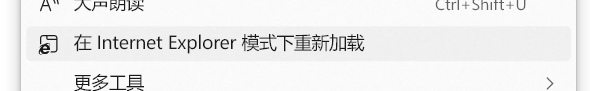
\includegraphics[width=7cm]{assets/Reload_in_IE_Mode.png}
  \caption{用 IE 模式重新加载}
  \label{Reload_in_IE_Mode}
\end{figure}

当然,对于 Windows 10 上的 Edge,也可以用这个方法进入「Internet Explorer 模式」,从而打开那些只支持 IE 浏览器的网站。

\section{国产套壳浏览器:众口难调,各取所需}

最后我们再来说说那些国产套 Chromium 壳的浏览器们。
这些浏览器数量庞大,其中不乏优质作品,也有许多流氓软件。
一般来说,大厂的产品如「360 安全浏览器」「360 极速浏览器」「QQ 浏览器」「搜狗高速浏览器」等,往往还属于比较可以接受的选择;
而「2345 加速浏览器」「极速浏览器」这种名不见经传甚至有流氓软件背景的产品,我们十分不建议使用。
下图是 360 安全浏览器的官网介绍。

\begin{figure}[htb!]
  \centering
  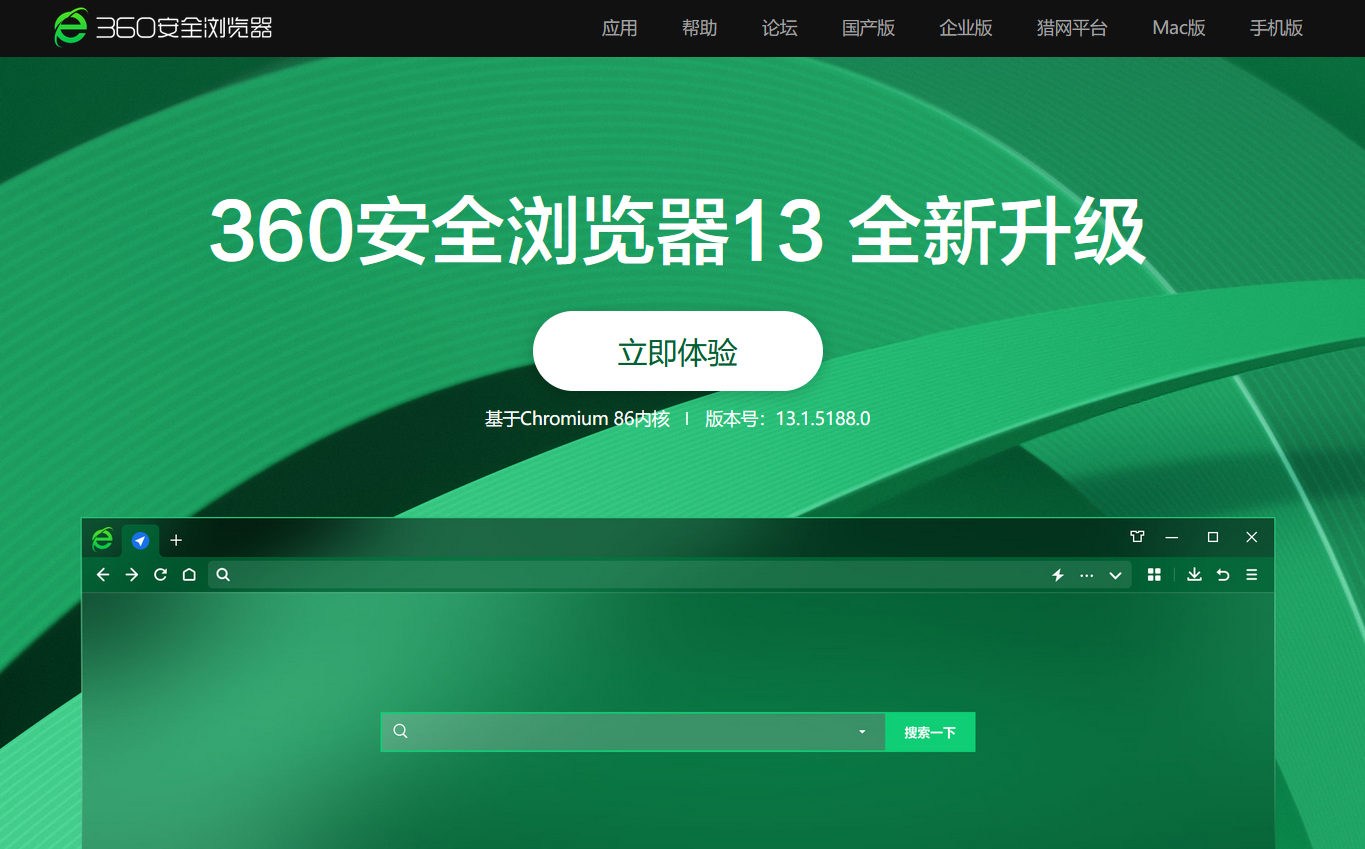
\includegraphics[width=9cm]{assets/360_se.png}
  \caption{360 安全浏览器}
  \label{360_se}
\end{figure}

这些国产套壳浏览器有着以下 Chrome 难以提供的功能:

\begin{itemize}
  \item 符合中国用户使用体验的同步功能。这些浏览器使用自家账号(例如 360 账号、QQ / 微信号等)登录,往往能与自家产品实现无缝联动,构成完整的体验。
  \item 为国内用户使用习惯打造的资讯推荐功能。这些浏览器一般有自己的首页,而首页上会根据国内用户的使用习惯定制、推荐新闻等推送。民间所谓「UC 体」其实就是「UC 浏览器」在首页推送中惯用的一种文体\CJKsout*{(震惊!这份电脑教程竟如此详细!)}。
  \item 各厂商为差异化推出的功能。例如,360 家族的浏览器总是主打「安全」,因为它们的主业是安全产品;QQ 浏览器集成了一些轻度办公的功能,这与腾讯文档等在线办公平台密不可分。
  \item ……
\end{itemize}

但国产套壳浏览器也有着一些令人讨厌之处。
首先是国产软件的通病——广告。
一些国产套壳浏览器会以弹窗等形式时不时向用户推送广告,这是十分令人厌烦的。
另一个问题是它们往往具有「捆绑推荐」的性质,如\nameref{basic-maintenance}中所提到的那样,如果你安装使用 QQ 浏览器,那它总是会在各种场合推荐腾讯的其他软件如「腾讯电脑管家」。
这很多时候并不是我们所愿意看到的。

总之,对于国产套壳浏览器,我们的建议是「众口难调,各取所需」,大家可以根据自己的实际需要和使用喜好来选用。

\section{设置你的「默认浏览器」}

所谓「默认浏览器」是指,当你在某处点击一个链接时,系统自动选择打开它的浏览器。
在\nameref{software-installation}中我们提到了「打开方式」的概念,默认浏览器便是与之类似的东西。

要把一款浏览器设置成你的默认浏览器,大体有两种方式:通过浏览器自身来设置,以及在系统中手动设置。

各大浏览器一般都给出了一键将自己设置成默认浏览器的入口。
我们只需要进入浏览器的「设置」「选项」等类似的页面,寻找「默认浏览器」的相关字眼,按提示操作即可完成设置。
例如,对于火狐浏览器,点选【≡】→【设置】就能看到默认浏览器的相关选项。

\begin{figure}[htb!]
  \centering
  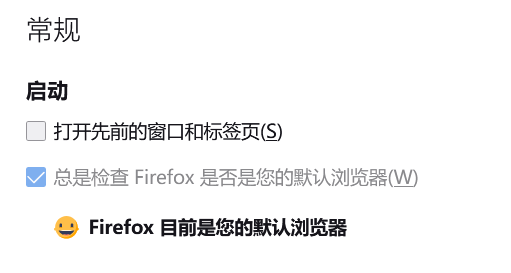
\includegraphics[width=7cm]{assets/Firefox_Default.png}
  \caption{火狐的「默认浏览器」设置}
  \label{Firefox_Default}
\end{figure}

在系统中手动选择默认浏览器则相对麻烦。
在 Windows 10 系统中,你可以通过打开系统【设置】→【应用】→【默认应用】→【Web 浏览器】来选定一款浏览器作为你的默认浏览器:

\begin{figure}[htb!]
  \centering
  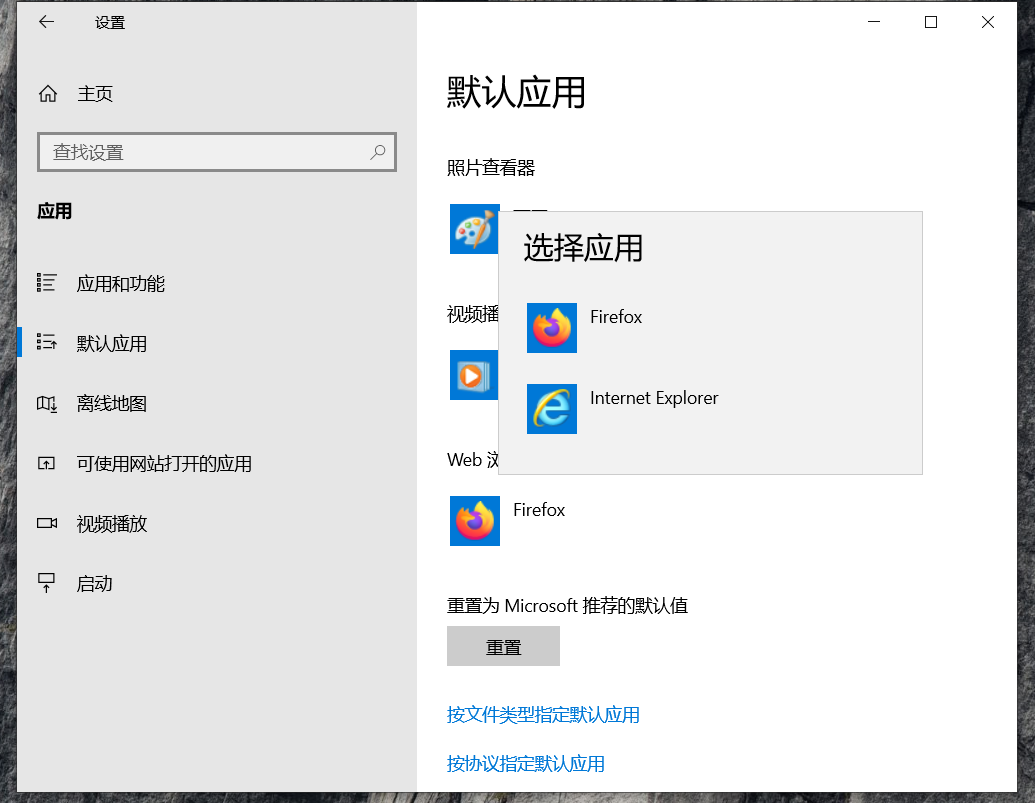
\includegraphics[width=9cm]{assets/Win_10_Default_Browser.png}
  \caption{Windows 10 系统的「默认浏览器」设置}
  \label{Win_10_Default_Browser}
\end{figure}

而在 Windows 11 中,微软为了强行推荐新 Edge 浏览器,将手动选择默认浏览器的功能砍掉了\CJKsout*{微软你真的坏事做尽},要想在系统中将一款浏览器设置成默认浏览器需要这样操作:

\begin{itemize}
  \item 打开系统【设置】→【应用】→【默认应用】,然后找到你希望设置成默认浏览器的浏览器,如图 \ref{Windows_11_default_browser}。
    \begin{figure}[htb!]
      \centering
      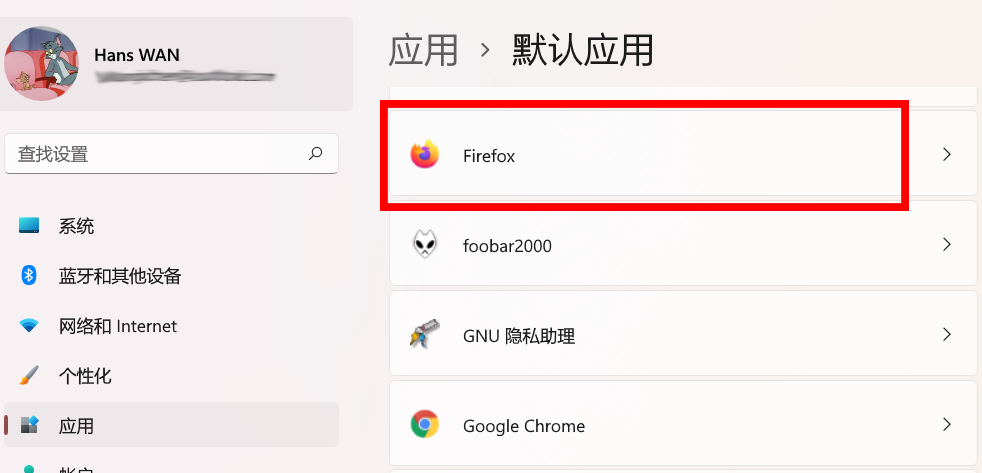
\includegraphics[width=8cm]{assets/Windows_11_default_browser.png}
      \caption{在 Windows 11 中选择默认浏览器}
      \label{Windows_11_default_browser}
    \end{figure}
  \item 点击后,将「\verb|.htm|」「\verb|.html|」「HTTP」「HTTPS」四个项目设置成这款浏览器(如图 \ref{Win_11_Change_Browser},图中只展示了其中的两个)。
    \begin{figure}[htb!]
      \centering
      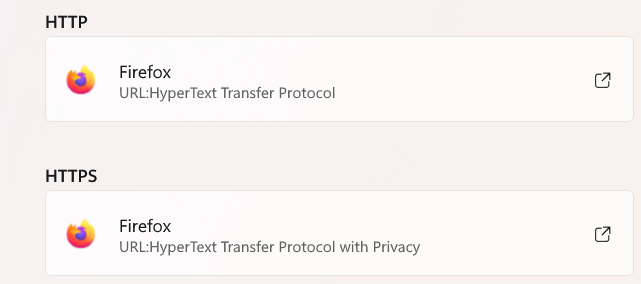
\includegraphics[width=8cm]{assets/Win_11_Change_Browser.png}
      \caption{在 Windows 11 中更改默认浏览器}
      \label{Win_11_Change_Browser}
    \end{figure}
\end{itemize}

\practice

\begin{enumerate}
  \item 根据「浏览器界的『血雨腥风』」一节的叙述,复述任意一款主流浏览器(火狐、IE、Chrome)的发展 / 兴衰史。
  \item 你正在用什么浏览器?你喜欢它的什么功能?如果你在阅读完这部分内容后想更换一款浏览器并长久使用,你会选择哪一款?
  \item 电脑里安装的浏览器是越多越好吗?为什么?
\end{enumerate}